\documentclass{article}
\usepackage{nips15submit_e, times}
\usepackage{amsmath}
\usepackage{amsfonts}
\usepackage{algorithm}
\usepackage{algorithmicx}
\usepackage{algpseudocode}
\usepackage{booktabs}
\usepackage{graphicx}
\usepackage{subfigure}
\usepackage{placeins}
\usepackage{enumerate}
\usepackage{diagbox}
\usepackage{tocbibind}

\title{Music Generation based on RNN and LSTM}
\date{February 2019}

\begin{document}

\maketitle
\begin{abstract}
In this report, we attempted  to use LSTM and vanilla RNN respectively to complete a ABC format music generation. First of all, we introduced the reason to use LSTM and RNN to solve this task instead of CNN and then introduced the architecture of out model. In the following, we conducted several comparison experiment. Firstly, based on our best hyper parameter, we generated 6  musics under $T=0.5,1,2$. Secondly, we plotted the training loss curve and validation loss curve to observe when the best model appeared. Thirdly, we compared the performance by changing the number of hidden nodes and found that for 150 neurons there exist a bounce up for validation set, which can be considered as an overfitted state. Fourthly, instead of using random sampling, we applied arg-max sampling to generate new music and concluded that it's hard to generate music following this rule. Fifthly, we replaced the model with vanilla RNN and found that vanilla RNN is worse than LSTM model. Last but not least, we generated a heatmap of the value corresponding to 20th hidden node and found that this neuron activated the body of the music.
\end{abstract}



\section{Introduction}
In the previous assignment, we solved several task using and Neural Networks and Convolutional Neural Networks. Both of their input h are not related to temporal. However, for those temporal related or order dependent input such as frames in a video and the words in a sentence, Multi-layer Neural Networks or Convolutional Neural Networks can't be used to solve. In this case, Recurrent Neural Network is the most fitful network. In this report, we will generate an innovative music by given a start sequence or even just one character.
\section{Methodology}
The basic RNN architecture shows in the. The green nodes represent the input. Normally, the input contains a sequence with a fixed length. The blue nodes represent the hidden nodes corresponding to different stages. The yellow nodes represent the output sequence. During the training, what we need to learn is the weights from the input to the hidden nodes, the weights from the hidden nodes to the outputs and the transfer from $\text{hidden}_{t-1}$ and $\text{hidden}_{t}$.
\begin{figure}[H]
\begin{center}
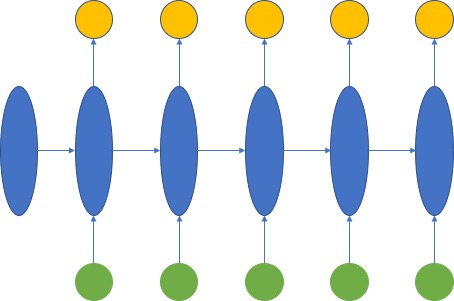
\includegraphics[scale=0.5]{image/RNN.jpg}
\end{center}
\caption{RNN Architecture}
\label{figure: RNN architecture}
\end{figure}
\subsection{Preproces Dataset}
The dataset we used is several corpuses of ABC format musics. Each of them are shown similar to Figure \ref{figure: ABC format}. The corresponding tune is shown in Figure \ref{figure: tune}.
\begin{figure}[H]
\begin{center}
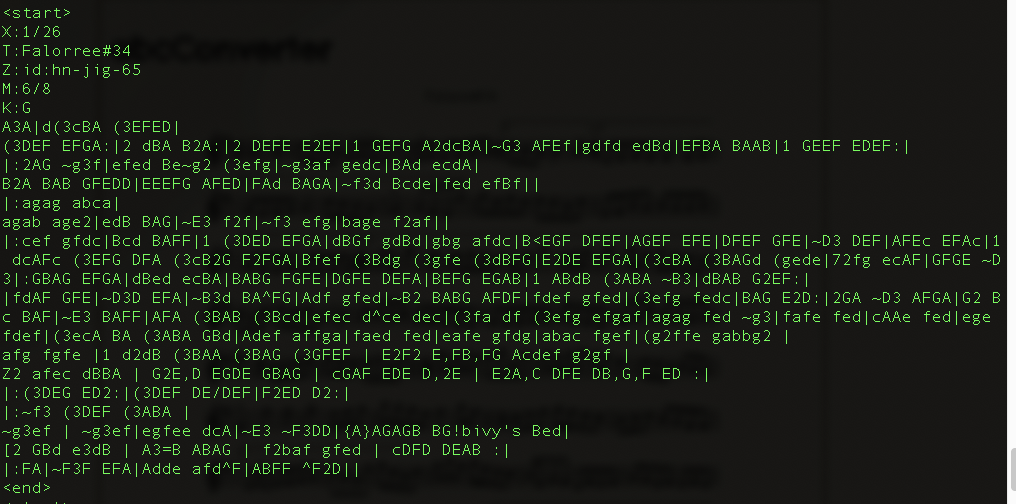
\includegraphics[scale=0.4]{image/music.png}
\end{center}
\caption{ABC format music sequence}
\label{figure: ABC format}
\end{figure}
\begin{figure}[H]
\begin{center}
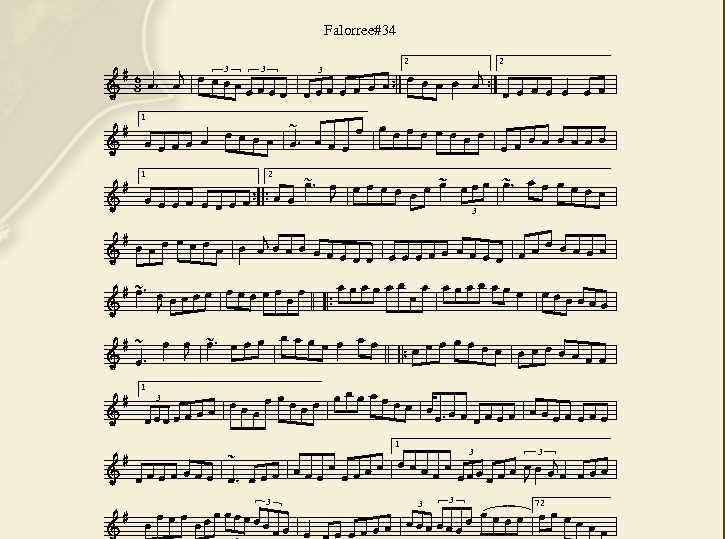
\includegraphics[scale=0.4]{image/tune.png}
\end{center}
\caption{Sample Music Sheet}
\label{figure: tune}
\end{figure}
First of all, in order to generate new sequences, it is necessary to know the vocabulary set which provides the model to choose characters to generate. Therefore, we read in the train.txt and found there are 93 characters in the training set and stored a mapping from the character to an index number of this character.
e are going to see how we can convert music from ABC notation to a playable format(.midi in this case) online.
\subsection{Design of Architecture}
Both RNN and LSTM need to specify a fixed length of input sequence. Therefore, we hard cut the input sequence into several pieces whose length is \textbf{Chunksize}. For example, we separated the sequence into ones with 100 characters. For those ones whose length are not 100, we padded them with space characters. The target should be the next stage of the input, which means the output is left shifted one char compared with input. For example, if the input is "abcd", then the target should be "bcde". For the hidden layer, we initially set each stage of them to be 100 nodes.
\subsection{Loss function}
For each stage, we need to determine what is the character for this stage. Therefore, the output should be activated by Softmax. Furtherlly, loss function should be the cross entrophy which is define as the following.
\begin{equation}
\begin{split}
    \text{Cross Entrophy}(Y,P) = -\sum_{c=1}^My_{\text{o,c}}log(p_{\text{o,c}})
\end{split}
\label{equation: weight_loss}
\end{equation}
\subsection{Music Generation}
After we have a trained model, it can be applied to generate new music. The model is feed with a prime start sequence and for each time the model should generate one character. We call this process as sampling. There are two ways to complete it. The first one is to generate the next character with the max probability. For example, there are 4 possible characters and the corresponding probability is $[0.1,0.2,0.6,0.1]$. The generated character is definitely the third character. However, this method brings a problem when one intermediate character is generated wrongly, the successive ones will also be unreasonable. To tackle this issue, another sampling method is introduced which is to generate randomly according to the distribution of the output but basically it is random. For example, for the above 4 characters' case, the model will flip a 4 side coin to decide which one should be generated whereas the probability of each side will be shown is following the distribution.
\section{Result}
\subsection{Generate 6 sample music pieces}

To fairly compare the sample music pieces generated by temperature sampling with different $T$, the same hyper parameters setting are used with chunk size 200, batch size 100 and hidden size 125 in different value of $T$.

Figure \ref{t_0.5_1}, \ref{t_0.5_nota_1}, \ref{t_0.5_2} and \ref{t_0.5_nota_2} show the ABC notation and music representation of $2$ sample music pieces with $T=0.5$.

\begin{figure}[H]
\begin{center}
  \centering
  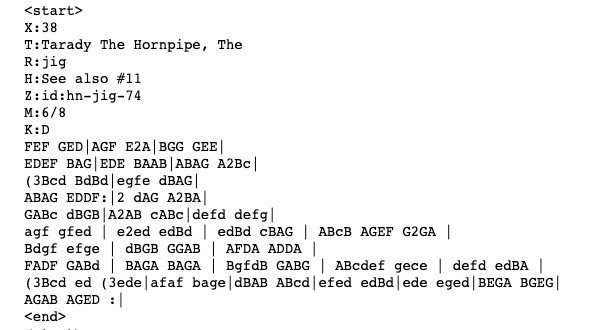
\includegraphics[width=5in]{image/t_05_1.png}
\end{center}
\caption{Generated Music 1 with $T=0.5$}
\label{t_0.5_1}
\end{figure}

\begin{figure}[H]
\begin{center}
  \centering
  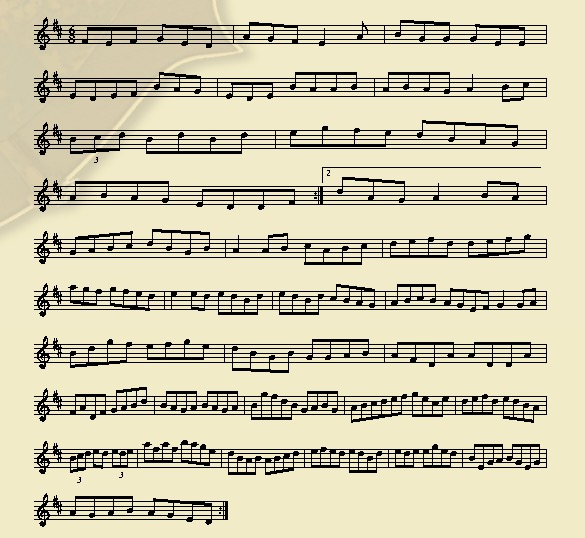
\includegraphics[width=4.5in]{image/t_05_1_nota.png}
\end{center}
\caption{Music 1 from Figure \ref{t_0.5_1} in standard music notation with $T=0.5$}
\label{t_0.5_nota_1}
\end{figure}

\begin{figure}[H]
\begin{center}
  \centering
  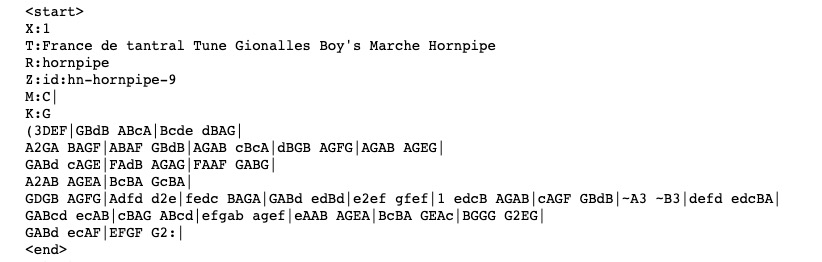
\includegraphics[width=5in]{image/t_05_2.png}
\end{center}
\caption{Generated Music 2 with $T=0.5$}
\label{t_0.5_2}
\end{figure}

\begin{figure}[H]
\begin{center}
  \centering
  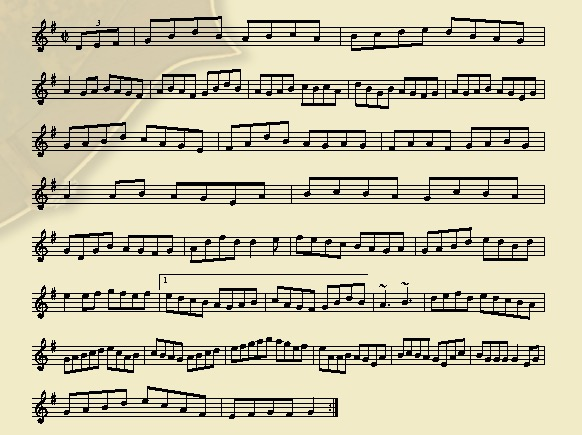
\includegraphics[width=4.5in]{image/t_05_2_nota.png}
\end{center}
\caption{Music 2 from Figure \ref{t_0.5_2} in standard music notation with $T=0.5$}
\label{t_0.5_nota_2}
\end{figure}

Figure \ref{t_1_1}, \ref{t_1_nota_1}, \ref{t_1_2} and \ref{t_1_nota_2} show the ABC notation and music representation of $2$ sample music pieces with $T=1$.

\begin{figure}[H]
\begin{center}
  \centering
  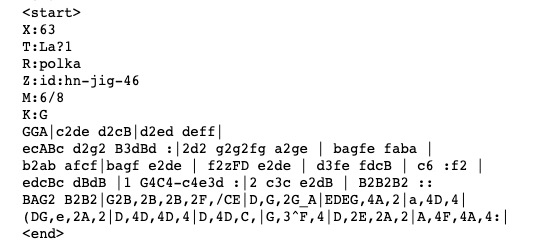
\includegraphics[width=5in]{image/t_1_1.png}
\end{center}
\caption{Generated Music 1 with $T=1$}
\label{t_1_1}
\end{figure}

\begin{figure}[H]
\begin{center}
  \centering
  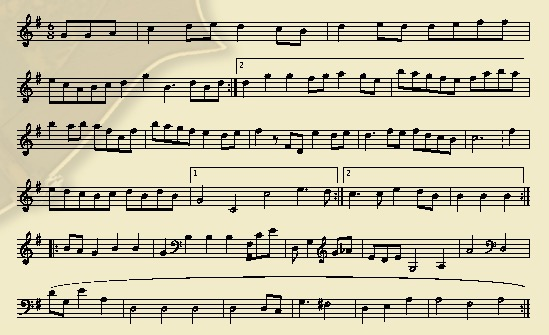
\includegraphics[width=4.5in]{image/t_1_1_nota.png}
\end{center}
\caption{Music 1 from Figure \ref{t_1_1} in standard music notation with $T=1$}
\label{t_1_nota_1}
\end{figure}

\begin{figure}[H]
\begin{center}
  \centering
  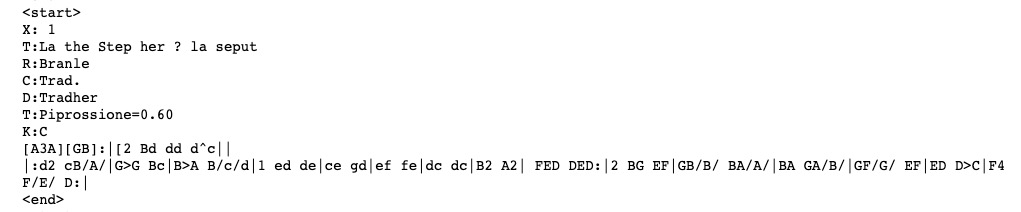
\includegraphics[width=5in]{image/t_1_2.png}
\end{center}
\caption{Generated Music 2 with $T=1$}
\label{t_1_2}
\end{figure}

\begin{figure}[H]
\begin{center}
  \centering
  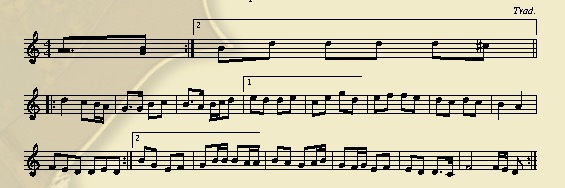
\includegraphics[width=4.5in]{image/t_1_2_nota.png}
\end{center}
\caption{Music 2 from Figure \ref{t_1_2} in standard music notation with $T=1$}
\label{t_1_nota_2}
\end{figure}

Figure \ref{t_2_1}, \ref{t_2_nota_1}, \ref{t_2_2} and \ref{t_2_nota_2} show the ABC notation and music representation of $2$ sample music pieces with $T=2$.

\begin{figure}[H]
\begin{center}
  \centering
  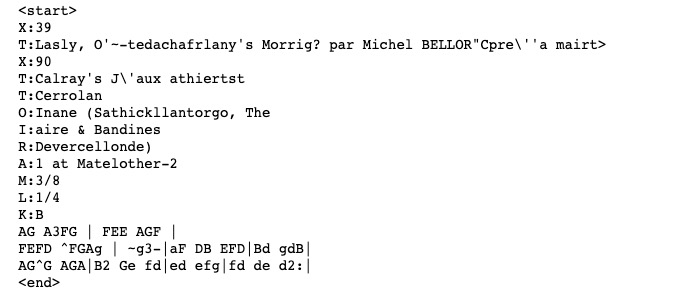
\includegraphics[width=5in]{image/t_2_1.png}
\end{center}
\caption{Generated Music 1 with $T=2$}
\label{t_2_1}
\end{figure}

\begin{figure}[H]
\begin{center}
  \centering
  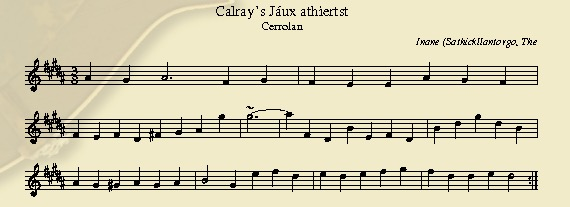
\includegraphics[width=4.5in]{image/t_2_1_nota.png}
\end{center}
\caption{Music 1 from Figure \ref{t_2_1} in standard music notation with $T=2$}
\label{t_2_nota_1}
\end{figure}

\begin{figure}[H]
\begin{center}
  \centering
  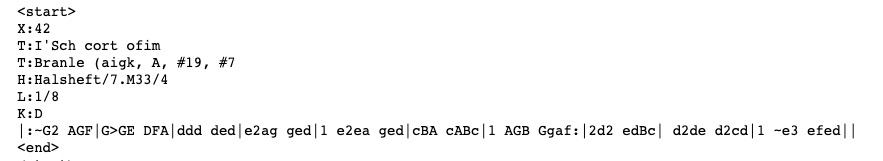
\includegraphics[width=5in]{image/t_2_2.png}
\end{center}
\caption{Generated Music 2 with $T=2$}
\label{t_2_2}
\end{figure}

\begin{figure}[H]
\begin{center}
  \centering
  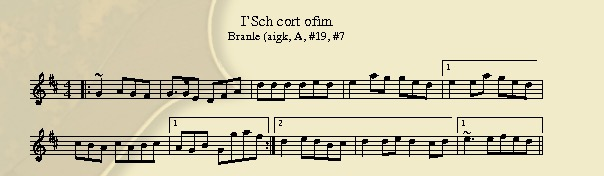
\includegraphics[width=4.5in]{image/t_2_2_nota.png}
\end{center}
\caption{Music 2 from Figure \ref{t_2_2} in standard music notation with $T=2$}
\label{t_2_nota_2}
\end{figure}

As we can see from Figure \ref{t_0.5_1} to Figure \ref{t_2_nota_2}, the larger the $T$ is, the sparser the musical tunes are. And the music generated by small value of $T$ sounds more rhythmic while music generated by large value of $T$ sounds more gentle and mild. We think that larger value of $T$ makes the model be uncentain about next character to be generated therefore generates less tunes to keep the continuity.

\subsection{Training loss and validation loss}

The configurations of hyper paramaters are as follow: chunk size 200, batch size 100 and hidden size 125.

Figure \ref{b: loss} shows the training loss and validation loss versus number of 100 epochs on data. It can be seen from figure that the training loss keeps decreasing while validation loss keeps reducing and reaches its minimum at roughly epoch 35 and then bounces up a little bit. The interesting thing we found during the experiment is that the minimum of validation loss with larger number of hidden units (300 hidden units with roughly 1.60 loss) is similar to smaller hidden units (125 hidden units with roughly 1.65 loss), which suggests that only increasing number of hidden units will not improve the performance a lot.

The blue line shows the test loss changing on test set. It can be seen from figure that the curve of test loss is much fluctuant compared to training and validation loss.

\begin{figure}[H]
\begin{center}
  \centering
  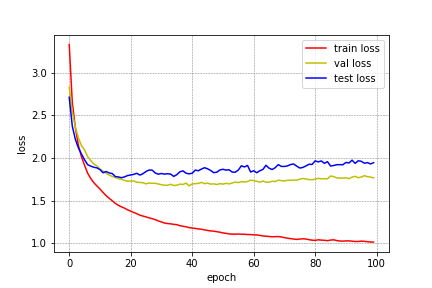
\includegraphics[width=3in]{image/b_lstm.png}
\end{center}
\caption{Training and validation loss of best model along with test loss.}
\label{b: loss}
\end{figure}

\subsection{Variation across number of neurons}

Figure \ref{various neurons} shows the training loss and validation loss versus number of epochs with different number of neurons in hidden layer. It can be seen from figure that the larger the number of neurons is, the smaller the training loss and validation are. It is noteworthy that the validation loss bounced up and kept raising after some specific epochs if the hidden layer has much more neurons and the curve is less smooth as well.

\begin{figure}[H]
\begin{center}
\begin{minipage}[l]{0.5\linewidth}
  \centering
  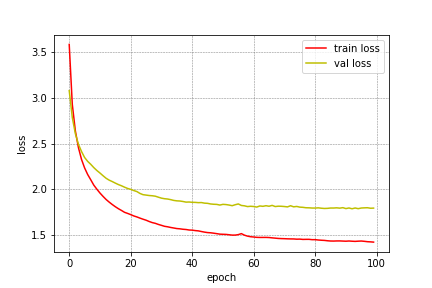
\includegraphics[width=3in]{image/c_hidden_size_50_lstm.png}
\end{minipage}
\begin{minipage}[c]{0.5\linewidth}
  \centering
  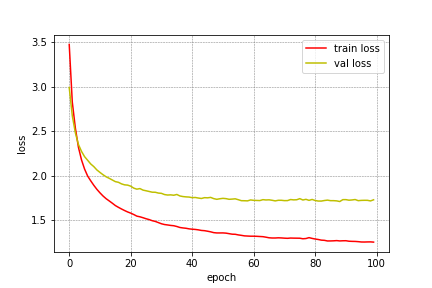
\includegraphics[width=3in]{image/c_hidden_size_75_lstm.png}
\end{minipage}
\begin{minipage}[r]{0.5\linewidth}
  \centering
  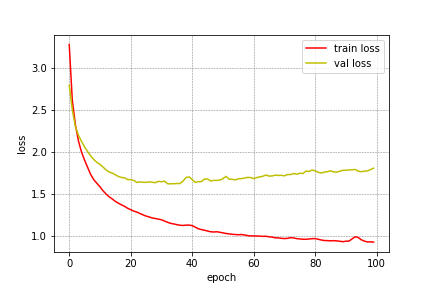
\includegraphics[width=3in]{image/c_hidden_size_150_lstm.png}
\end{minipage}
\end{center}
\caption{Training loss and validation loss versus 100 epochs with different number of neurons. \textbf{Top:} 50 neurons. \textbf{Middle:} 75 neurons. \textbf{Bottom:} 150 neurons.}
\label{various neurons}
\end{figure}

\subsection{Arg-max Sampling}

The sequence generated by temperature based sampling is complete and can be converted to musical tune and the music sounds pretty rhythmic and natural. Figure \ref{d: argmax} shows the sequence generated by arg-max. It can be seen from figure that arg-max keeps generating the same sequence given the start token $<start>$ which makes sense because arg-max generates the next character with the highest probability everytime and the start token is always be $<start>$ which means that arg-max will always generate the same output sequence. We converted the sequence into music and listened to it to find out that the music is less rhythmic and sounds mild and pale.

\begin{figure}[H]
\begin{center}
  \centering
  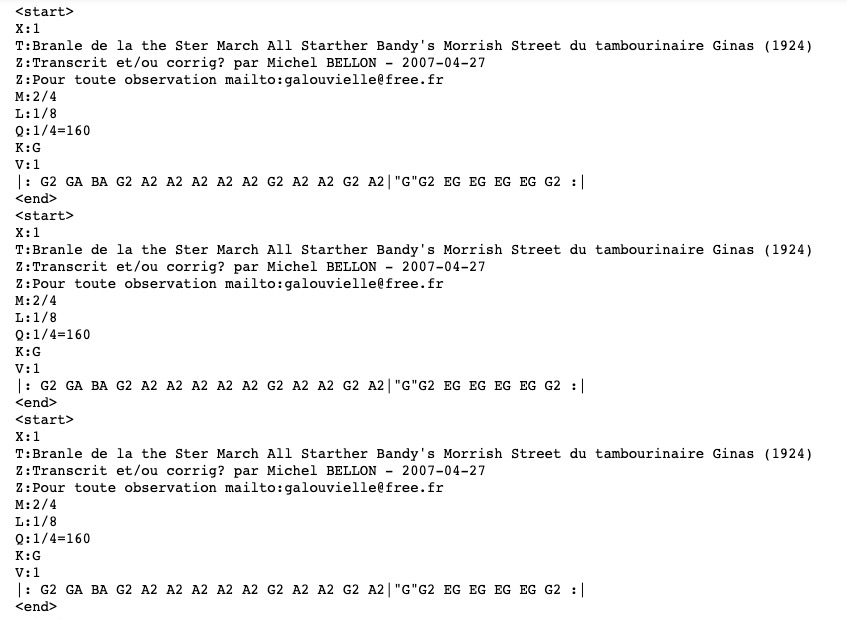
\includegraphics[width=5in]{image/d_argmax.png}
\end{center}
\caption{Sequence generated by arg-max.}
\label{d: argmax}
\end{figure}

\subsection{vanilla RNN}

To fairly compare the training loss and validation loss for LSTM and vanilla RNN, we fixed the same hyper paramaters with 100 hidden units, 200 chunk size, 100 batch size, Adam Optimizer and 0.01 learning rate.

Figure \ref{lstm vs vanilla} shows the comparison of training loss and validation loss between LSTM and vanilla RNN. It is apparent that the performance of vanilla RNN is worse than LSTM. Both the training loss and validation loss of LSTM are way smaller than vanilla RNN. Vanilla RNN mostly remembers what the later tune characters and does not take longer dependencies into consideration therefore might forget previous tunes. LSTM instead is able to learn what previous tune to remember and forget so the music generated by LSTM is more natural and precise.

\begin{figure}[H]
\begin{center}
  \centering
  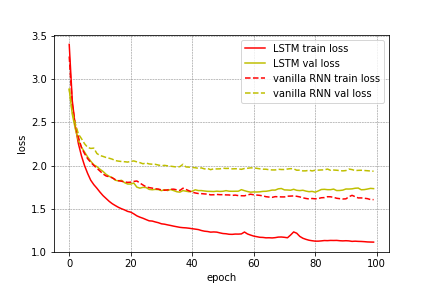
\includegraphics[width=3in]{image/e_lstm_vanilla.png}
\end{center}
\caption{Training and validation loss of LSTM and vanilla RNN.}
\label{lstm vs vanilla}
\end{figure}
\subsection{Feature Evaluation}
In this subsection, we are attempting to observe the activation value of one hidden node for the generated sequence. In this way, we can utilize the heatmap to reflect some interesting features of each of the hidden node. One of the activation heatmaps of the 20th hidden node across all the characters is shown in Figure \ref{figure: heatmap}.
\begin{figure}[H]
\begin{center}
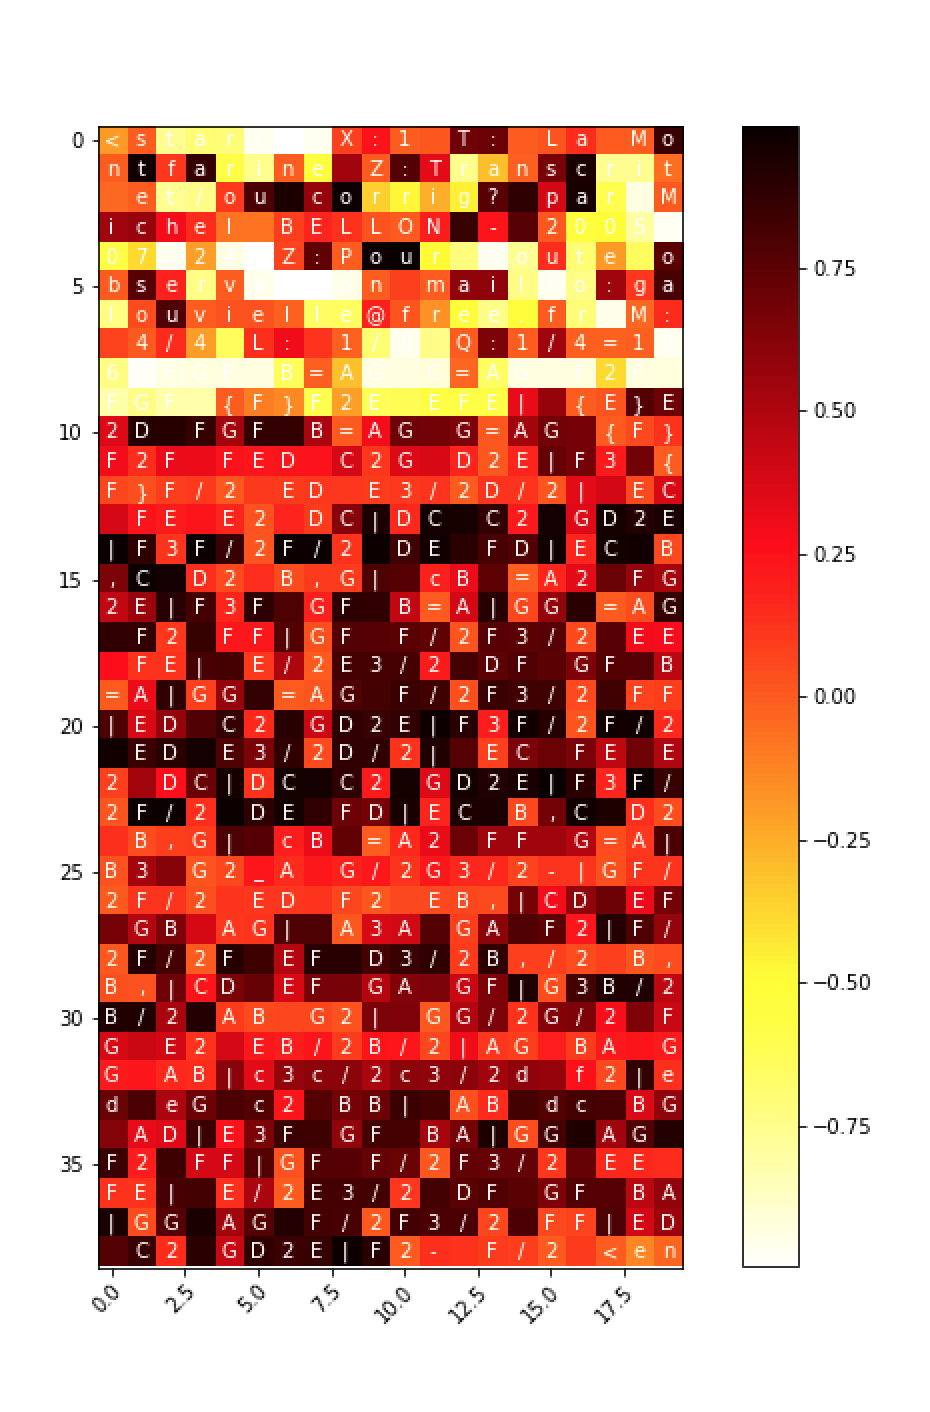
\includegraphics[scale=0.5]{image/heatmap.png}
\end{center}
\caption{Heatmap showing that this particular neuron fires for the body}
\label{figure: heatmap}
\end{figure}
From the heatmap, we can find that the values for the body of the sequence was activated and the value of header was low. Therefore, it can intuitively show that this specific neuron is for the purpose of identifying the body of a music.

\section{Contribution}
\paragraph{Guanghao Chen} Both Qimin and Guanghao first implemented LSTM model and we found his model's performance was better, so we adopted his finally. Besides, Guanghao generated the heatmap of the model and composed the abstraction, introduction, methodology and heatmap generation part in the report.

\paragraph{Qimin Chen} Qimin implemented the LSTM model and fined tune the networks to find the best model. For the report, we discussed the results together and Qimin wrote the music generation by temperature based sampling part.

\paragraph{Yunfan Chen} We discussed the results together and Yunfan plotted all the training loss, validation loss and test loss. Also Yunfan did the experiments of changing number of neurons in hidden layer and wrote the corresponding part of report.

\paragraph{Ke Xiao} We discussed the results together and Ke implemented the vanilla RNN and music generation by arg-max sampling. Ke wrote the qualitatively comparison of temperature sampling and arg-max sampling and the comparison of LSTM and vanilla RNN of the report.


\end{document}
